\documentclass[12pt]{report}
	\usepackage[margin=1in, top=1.5cm]{geometry}
	\usepackage[hidelinks, linktoc=all, pagebackref, russian]{hyperref}
	\usepackage{indentfirst}
    \usepackage{subcaption}
   	\usepackage[superscript,biblabel]{cite}
    \usepackage[font=small,labelfont=bf]{caption}
    \usepackage{abstract}
    \usepackage{mathtools}
    \usepackage{cleveref}
    \setlength{\parskip}{0.1cm}   
	\setlength{\parindent}{0.7cm}
    \usepackage{graphicx} % Used to insert images
    \usepackage{adjustbox} % Used to constrain images to a maximum size 
   	\usepackage{color} % Allow colors to be defined
    \usepackage{enumerate} % Needed for markdown enumerations to work
    \usepackage{geometry} % Used to adjust the document margins
    \usepackage{amsmath} % Equations
    \usepackage{amssymb} % Equations
    \usepackage[mathletters]{ucs} % Extended unicode (utf-8) support
    \usepackage[utf8x]{inputenc} % Allow utf-8 characters in the tex document
    \usepackage{fancyvrb} % verbatim replacement that allows latex
    \usepackage{grffile} % extends the file name processing of package graphics 
                         % to support a larger range 
    % The hyperref package gives us a pdf with properly built
    % internal navigation ('pdf bookmarks' for the table of contents,
    % internal cross-reference links, web links for URLs, etc.)
    \usepackage{longtable} % longtable support required by pandoc >1.10


 	
 \renewcommand{\figureautorefname}{Fig.}%
\renewcommand*\thesection{\arabic{section}}
\DeclarePairedDelimiter\bra{\langle}{\rvert}
\DeclarePairedDelimiter\ket{\lvert}{\rangle}
\DeclarePairedDelimiterX\braket[2]{\langle}{\rangle}{#1 \delimsize\vert #2}
\newcommand{\rbrkt}[1]{\left( #1 \right)}
\renewcommand*{\backreftwosep}{ and~}
\renewcommand*{\backreflastsep}{ and~}
\renewcommand*{\backref}[1]{}
\renewcommand*{\backrefalt}[4]{%
\ifcase #1 %
\relax%
\or
(referenced on p. [#2])%
\else
(referenced on p. [#2])%
\fi
}

\numberwithin{equation}{section}
\setcounter{tocdepth}{3}


\title{Reverse engineering of the XMon qubits}

\graphicspath{{Pictures/}}

\begin{document}
\maketitle

\chapter{Design of the coupling to readout resonator}

\section{Equations for quality factors}

The observed quality factor of a microwave transmission line resonator (TLR) $Q_l$ (loaded quality factor) can be calculated as a sum of two parts -- the internal and external quality factors. The internal quality factor $Q_i$ describes how excitations leave the resonator in the absence of coupling to the transmission line, so damping in this case comes from the internal defects of the resonator itself. When, however, the resonator is coupled to the external circuitry with some active resistance, the damping is enhanced and the observed Q-factor is reduced according to the following formula:
\begin{equation}
Q_l^{-1} = Q_i^{-1}+Q_e^{-1},
\label{eq:qfactor}
\end{equation}
where $Q_e$ is determined by the value of the externally connected resistance and the way of its connection.

\begin{figure}
\captionsetup[subfigure]{width = 0.9\textwidth, justification=normal}
\centering
\begin{subfigure}[t]{0.48\textwidth}
\centering
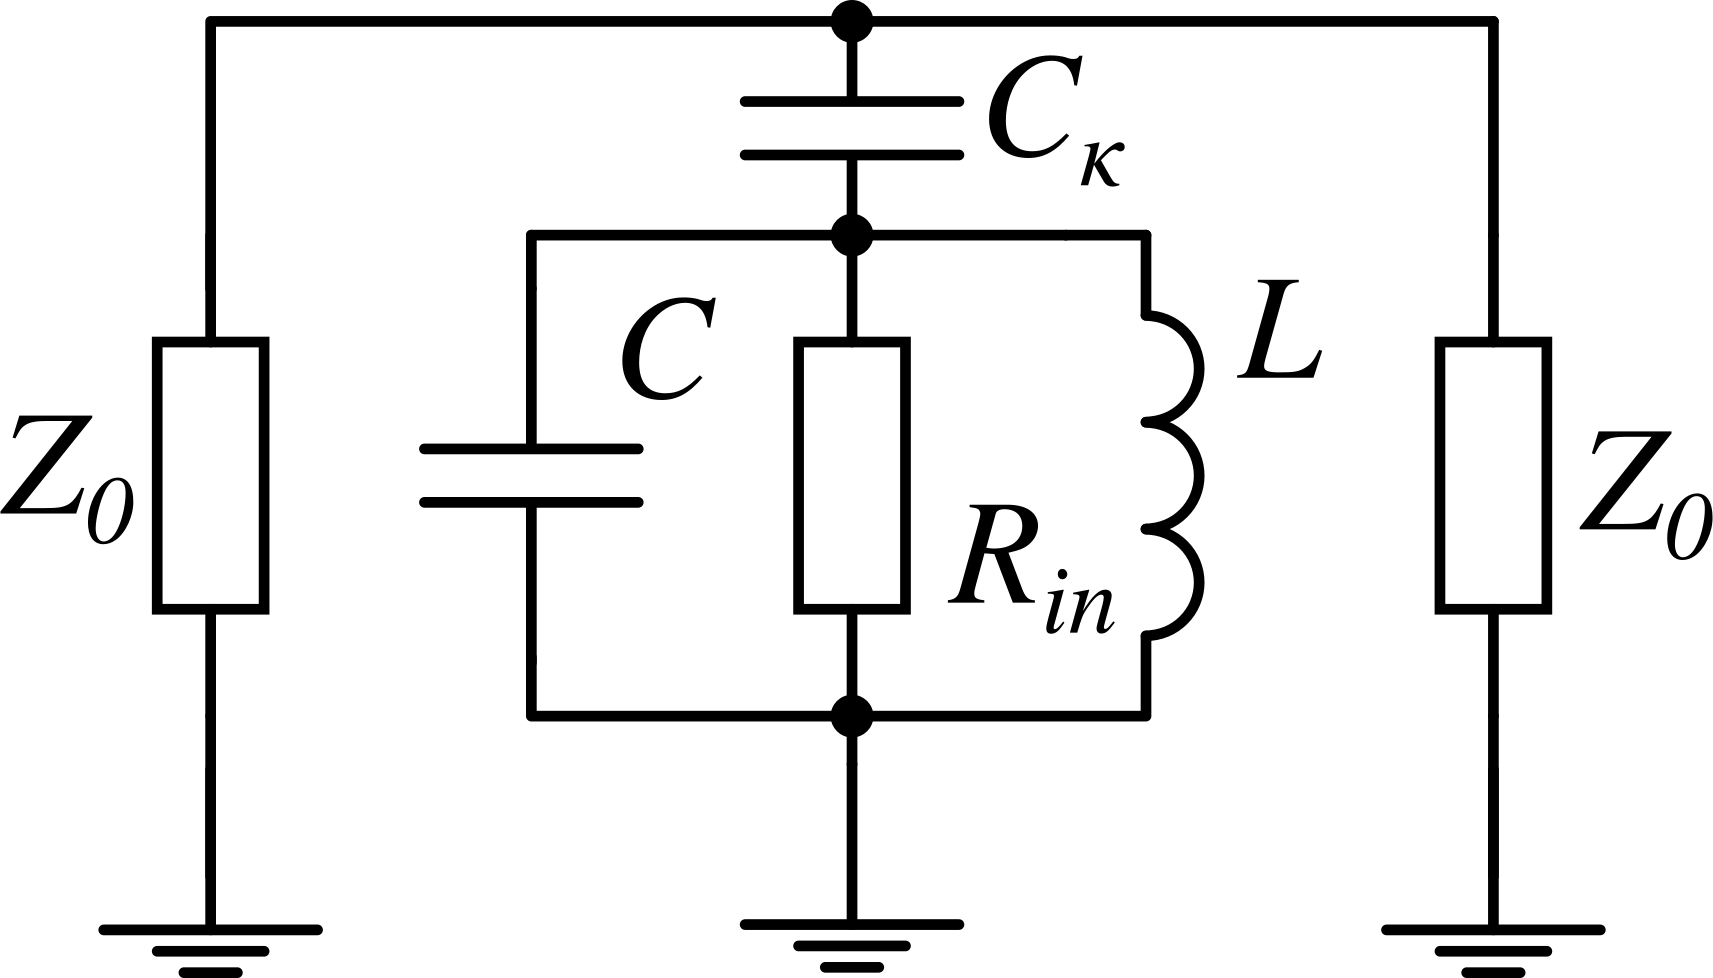
\includegraphics[width=0.9\textwidth]{resonator}
\caption{Real world circuit configuration.}
\end{subfigure}
\begin{subfigure}[t]{0.48\textwidth}
\centering
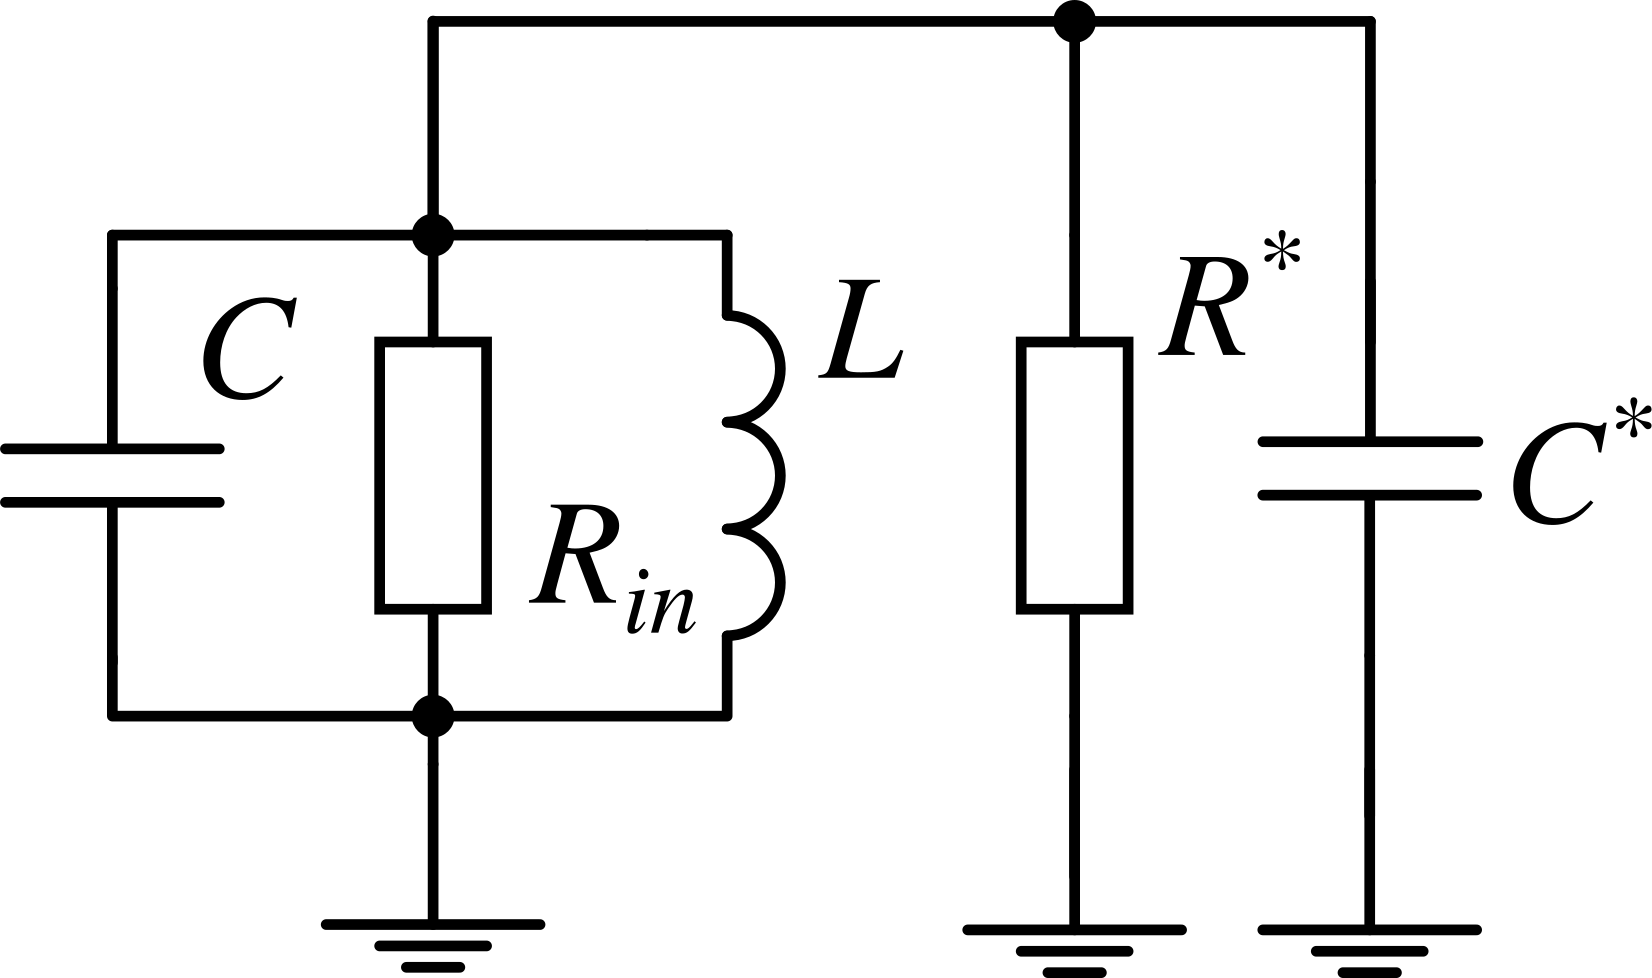
\includegraphics[width=0.9\textwidth]{resonator_equiv}
\caption{Norton equivalent of (a).}
\end{subfigure}

\caption{Equivalent circuit for a $\lambda/4$ TLR, capacitively coupled to the transmission line from the system's point of view.}
\label{fig:resonator_equiv}
\end{figure}

The common way of connection is the capacitive coupling $C_\kappa$ to the transmission line, as depicted on the equivalent scheme of the circuit in \autoref{fig:resonator_equiv}~(a). To draw the equivalent scheme of the circuit one needs first to determine the type of the resonance for the chosen TLR\cite{pozar2012}. In the studied design the resonators are $\lambda/4$ thus the equivalent for each of them is the parallel RLC resonator, where $C$ and $L$ are equivalent capacitance and inductance and $R=R_{in}$ characterises the internal dissipation. Its $Q_i  = \omega_0	C R_{in}$ where $\omega_0 = \sqrt{1/LC}$ can be calculated from the definition when no external impedance is connected.
 
The external Q-factor can be derived in a bit more complicated way\cite{Goppl2008}. We can transform the circuit on the \autoref{fig:resonator_equiv}~(a) to explicitly include the external parameters in the internal ones. To do so one needs to convert the series connection of the coupling capacitor and the characteristic impedances into parallel, as done on the \autoref{fig:resonator_equiv}~(b). The $R^*$ and $C^*$ impedances should be chosen in such a way that total impedance of the external circuit was the same as before the transformation. To achieve this $R^*$ and $C^*$ must be calculated as follows:
\begin{gather}
R^{*} = \frac{1+\omega^2 C_\kappa^2 (Z_0/2)^2}{\omega^2 C_\kappa^2 (Z_0/2)	} \\
C^{*} = \frac{C_\kappa}{1+\omega^2 C_\kappa^2 (Z_0/2)^2} \approx C_\kappa (\text{for our case}). \label{eq:C_ast}
\end{gather}
From this and \autoref{fig:resonator_equiv}~(b) it is simple to write down the expression for the external and loaded quality factors:
\begin{gather}
Q_e = \omega (C+C^{*}) R^{*} \\
Q_l = \omega (C+C^{*})  \frac{1}{1/R^{*}+1/R_{in}}. \label{eq:Q_l}
\end{gather}
If one considers $C^{*} \ll C$ the above expressions readily justify \eqref{eq:qfactor}. The values been used in the simulations are: $C = 350$ fF, $L = 2$ nH, $R_{in}=10^7$ Ohm, $Z_0 = 50$ Ohm.

\begin{figure}
\centering
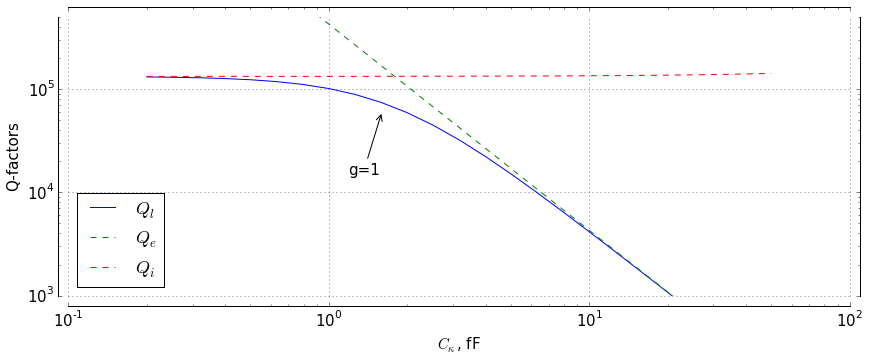
\includegraphics[width=0.9\textwidth]{q-factors}
\caption{Q-factors dependence on $C_\kappa$ according to \eqref{eq:Q_l}.}
\end{figure}



\begin{figure}
\centering
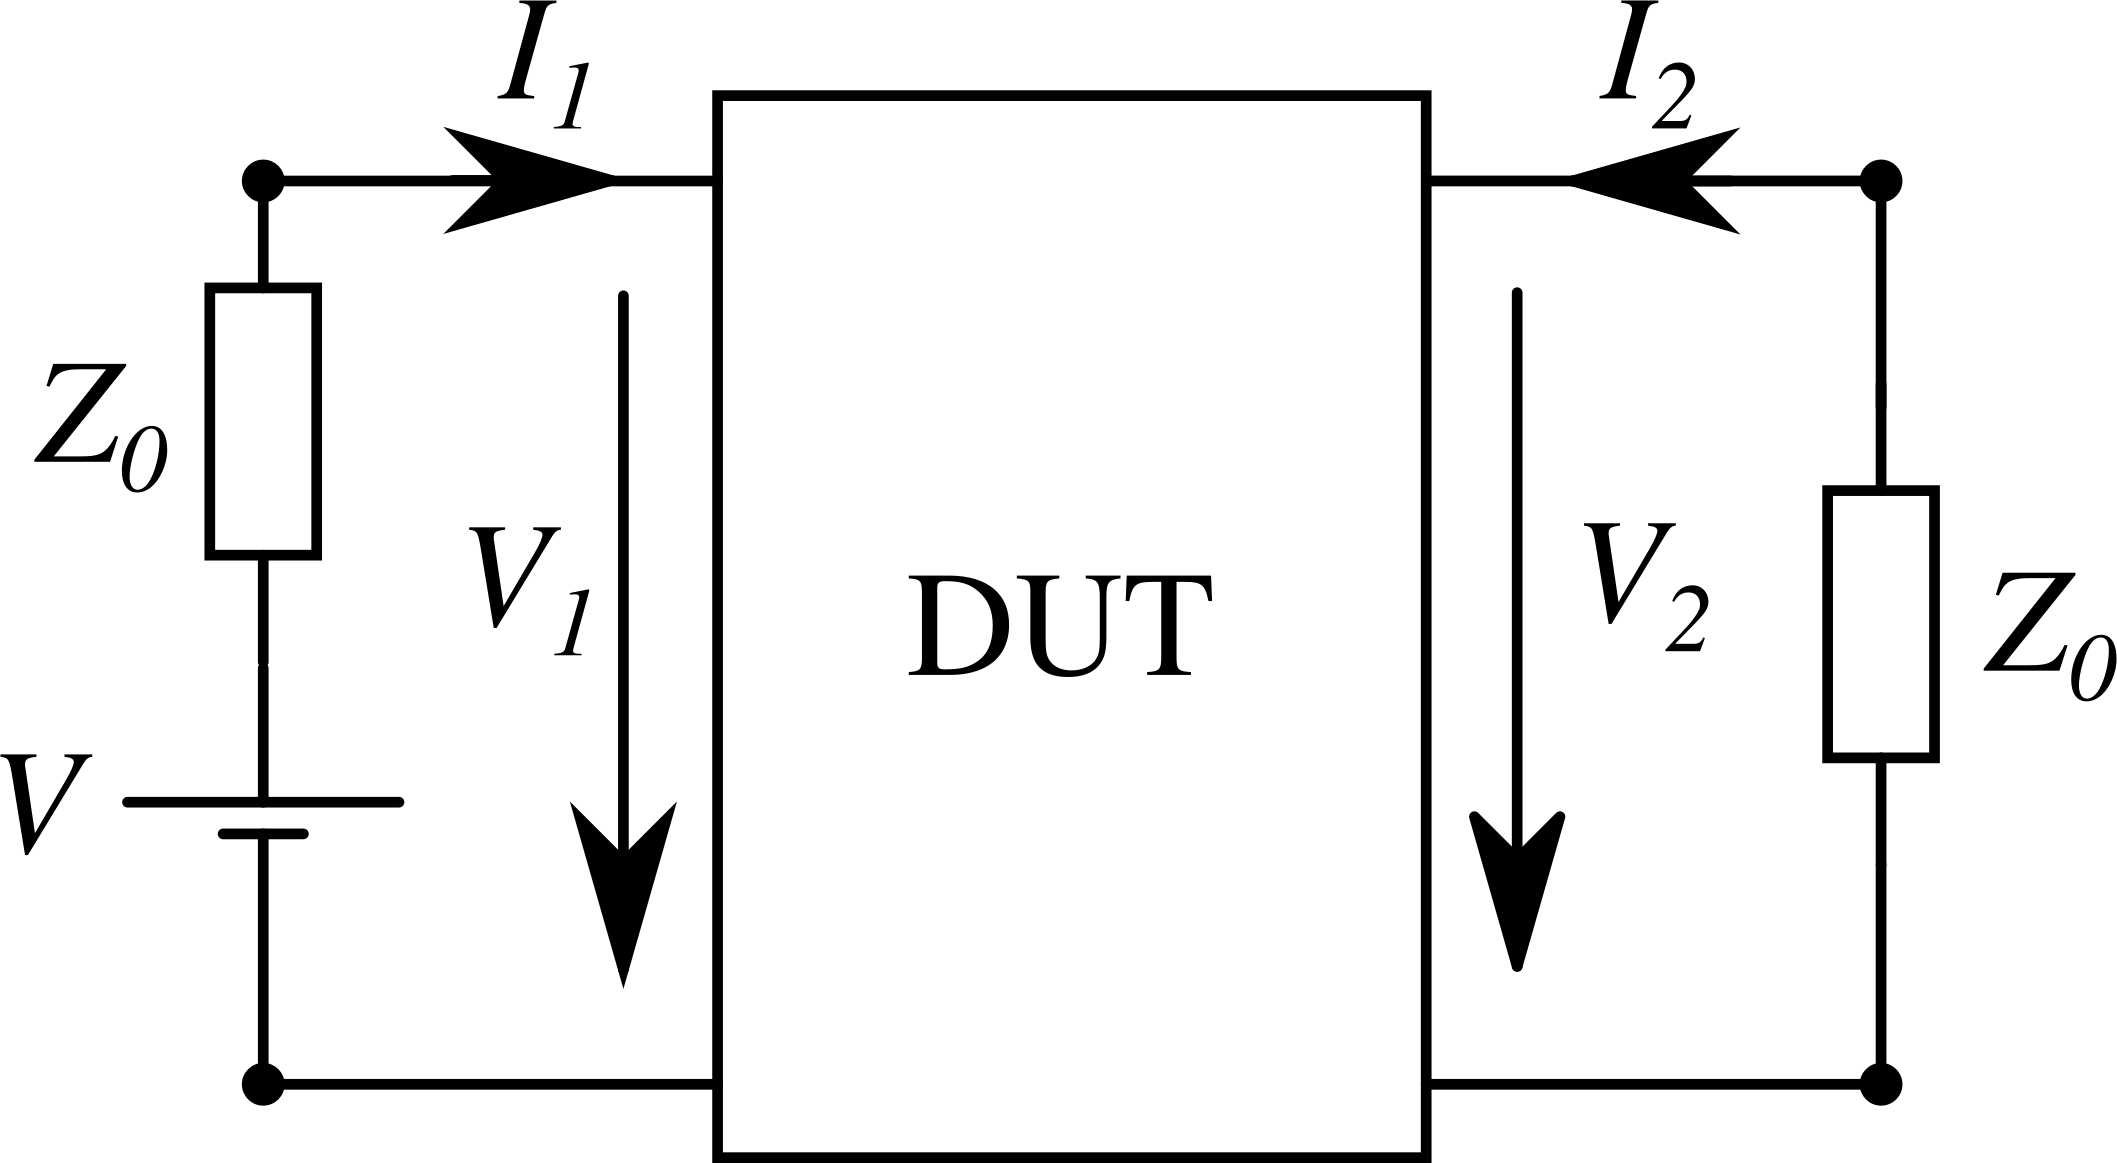
\includegraphics[width=0.5\textwidth]{tl_scheme_general}
\caption{A scheme for the two-port network.}
\label{fgeneral2port}
\end{figure}

\section{S-parameters}

\subsection{Introduction}

In the following two subsections we will discuss the scattering matrix for the two different configurations of resonator coupling. Generally, a two-port microwave device under test can be drawn like in \autoref{fgeneral2port}. For such system it is possible to calculate different 2 by 2 matrices, which bind together voltages and currents on the ports 1 and 2.

To calculate S-parameters one needs to treat voltages and currents, which can be calculated from Kirchhoff's laws, as a sum of the incident and reflected components (``+'' corresponds to the incident wave and ``$-$'' to the reflected wave):
\begin{gather*}
V_{1,2} = V_{1,2}^+ + V_{1,2}^- \\
I_{1,2} = I_{1,2}^+ - I_{1,2}^- = \frac{V_{1,2}}{Z_0},
\end{gather*}
where the difference in the second expression comes from telegrapher's equations. Solving these with respect to incident and reflected components, one can get
\begin{equation*}
V_{1,2}^\pm = \frac{1}{2}(V_{1,2} \pm Z_0 I_{1,2}).
\end{equation*}
From this, finally, S-parameters are defined:
\begin{equation}
\rbrkt{\begin{matrix}
V_1^- \\
V_2^-
\end{matrix}} = 
\rbrkt{\begin{matrix}
S_{11} & S_{12} \\
S_{21} & S_{22}
\end{matrix}}
\rbrkt{\begin{matrix}
V_1^+ \\
V_2^+
\end{matrix}}.
\end{equation}
However, it's often more convenient to use indirect methods of calculating S-parameters, for example, to extract them from $ABCD$-matrix.

\subsection{Coupled (shunting) design}
For a coupled design one needs to treat the resonator as a shunt in the transmission line as in \autoref{fig:shunted_tl}. Then there are two similar ways to calculate the S-matrix. First is intuitive but is not valid for every configuration. Transmission and reflection parameters are defined\cite{Kiselev2013} below (the second formula is valid only for the ``shunt'' configuration, no series elements are allowed in the line):
\begin{gather}    
\Gamma = \frac{Z_{eff} - Z_{0}}{Z_{eff} + Z_{0}} = S_{11} = S_{22} \label{eGamma}\\
T = \frac{2Z_{eff}}{Z_{eff}+Z_0} \overset{!}{=} S_{21} = S_{12}, \label{eT}
\end{gather}
where $Z_{eff} = Z_0 || Z_{shunt}$ and the equalities between S-parameters hold due to the symmetry.\begin{figure}[h]
\centering
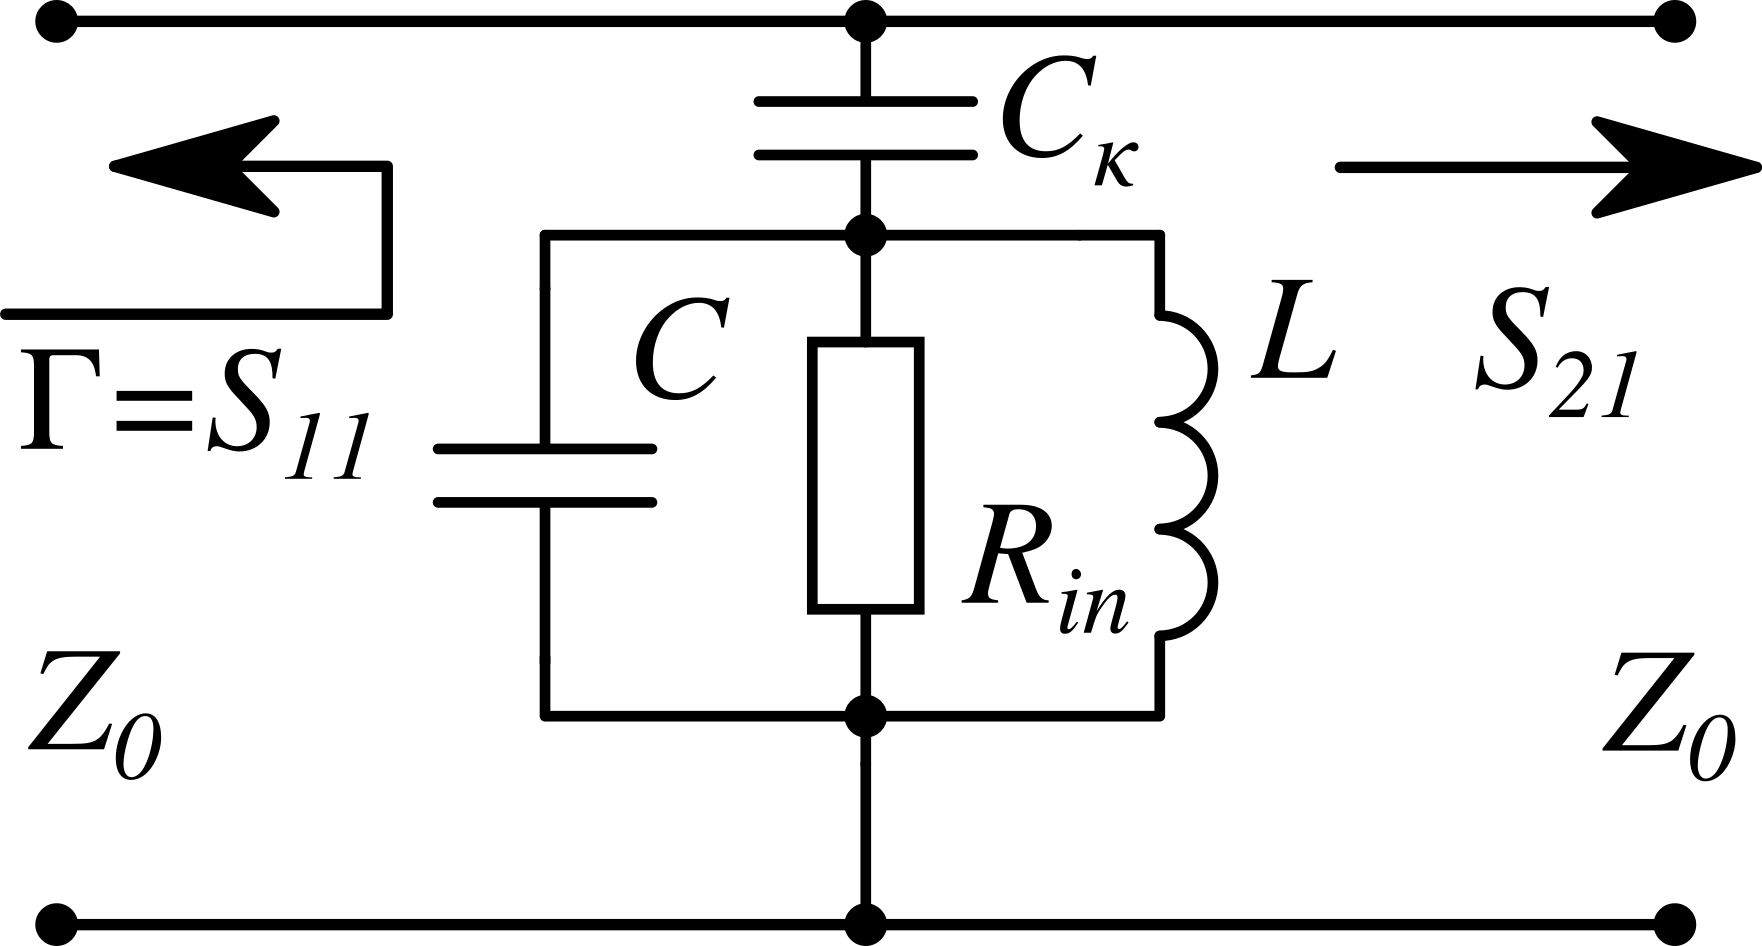
\includegraphics[width=0.5\textwidth]{tl_scheme}
\caption{The shunted transmission line. This is \autoref{fig:resonator_equiv}~(a)  from the observer's point of view.}
\label{fig:shunted_tl}
\end{figure}
\begin{figure}[h]
\centering
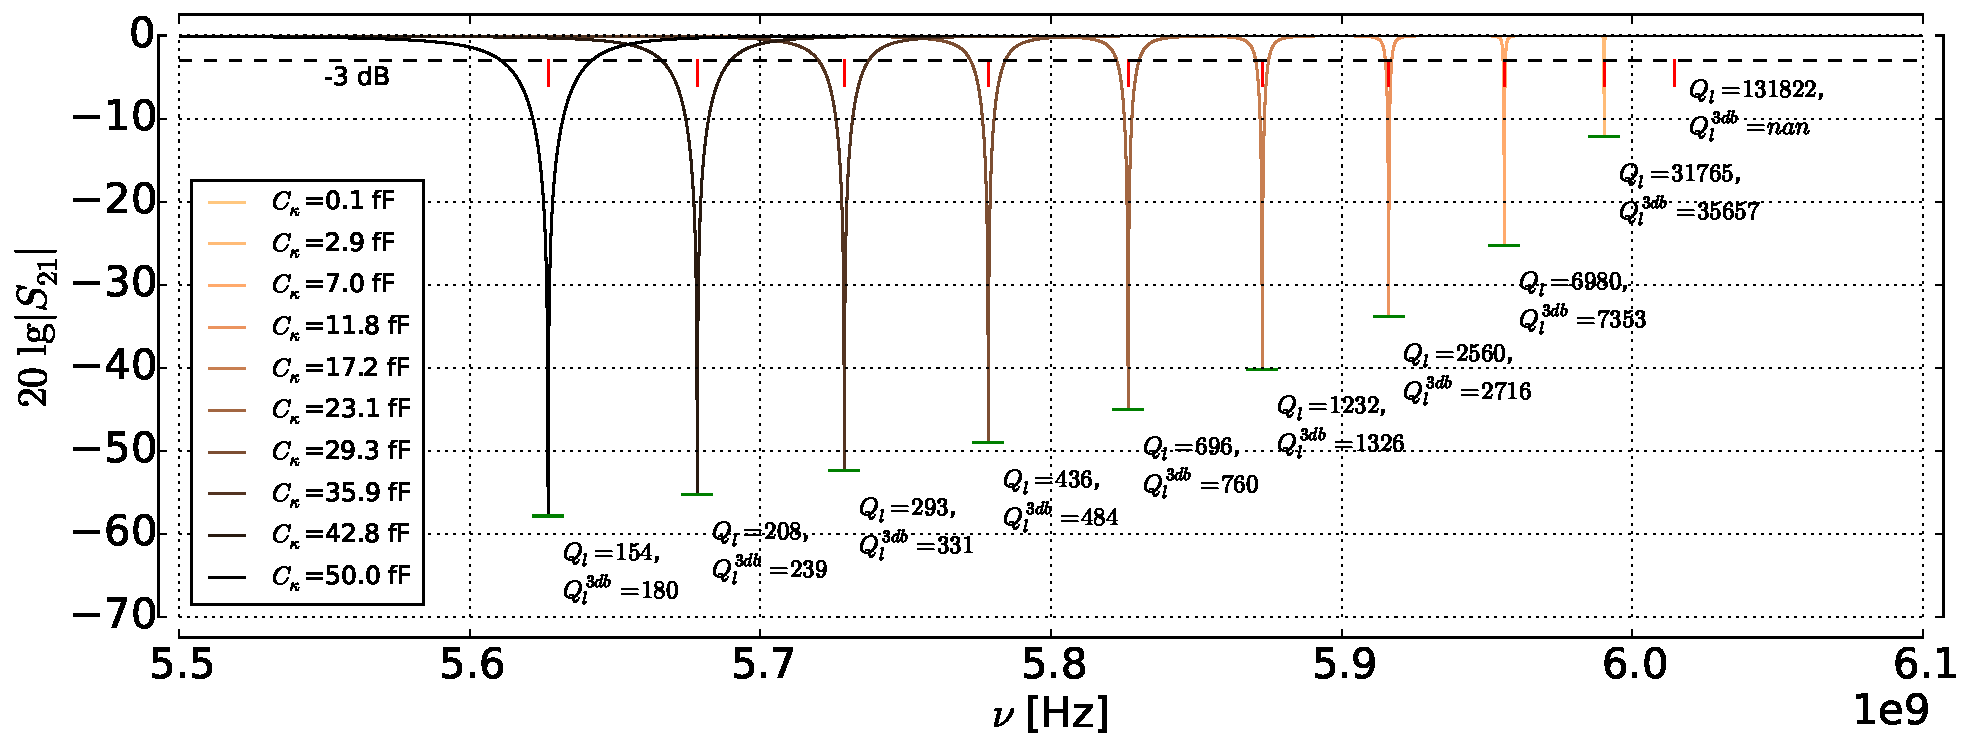
\includegraphics[width=0.99\textwidth]{S21s}
\caption{ $S_{21}$ parameters simulated with \eqref{eq:S21} for different coupling strengths. The loaded quality factors are calculated with \eqref{eq:Q_l} and with ``3db''-method. The red dashes show the values of expression $\sqrt{1/L(C+C_k)}$ according to \autoref{fig:resonator_equiv}~(b), the green ones show the theoretically predicted depths.}
\label{fig:S21s}
\end{figure}

Another way (totally reliable) is to calculate $ABCD$ matrix or impedance matrix and convert it to the S-matrix with corresponding formulae\cite{pozar2012}. From both this approaches the simplified expressions for the S-parameters follow:
\begin{gather}
S_{11} = -\frac{Z_0}{1 + 2Z_{shunt}/Z_0} = S_{22} \\
S_{21} = \frac{1}{1+Z_0/2Z_{shunt}} = S_{12} \label{eq:S21}
\end{gather}
The second expression is plotted in \autoref{fig:S21s} along with the loaded quality factors calculated by \eqref{eq:Q_l} and by ``3db''-method. It can be seen that with increase of capacitance resonance frequency shifts down, which is expected according to \autoref{fig:resonator_equiv}~(b) and \eqref{eq:C_ast} and $Q_l$ decreases.

In \autoref{fig:S21s} the resonance frequencies calculated from the equivalent circuit in \autoref{fig:resonator_equiv}~(b) are shown along with the analytically calculated depths of the peaks:
\begin{equation}
\min_f S_{21} = \frac{2 L \left(C + C_{\kappa}\right)}{\sqrt{C_{\kappa}^{2} L Z_{0}^{2} \left(C + C_{\kappa}\right) + \left(2 (C+C_\kappa) L + C_{k}^{2} R_{in} Z_{0} \right)^{2}}}
\end{equation}

\subsection{Embedded (series) design}

For the embedded resonator it's possible to draw a similar equivalent circuit as for the ``shunt'' design\cite{Goppl2008}. It is depicted in \autoref{fseries_tl}. 

\begin{figure}[h]
\centering
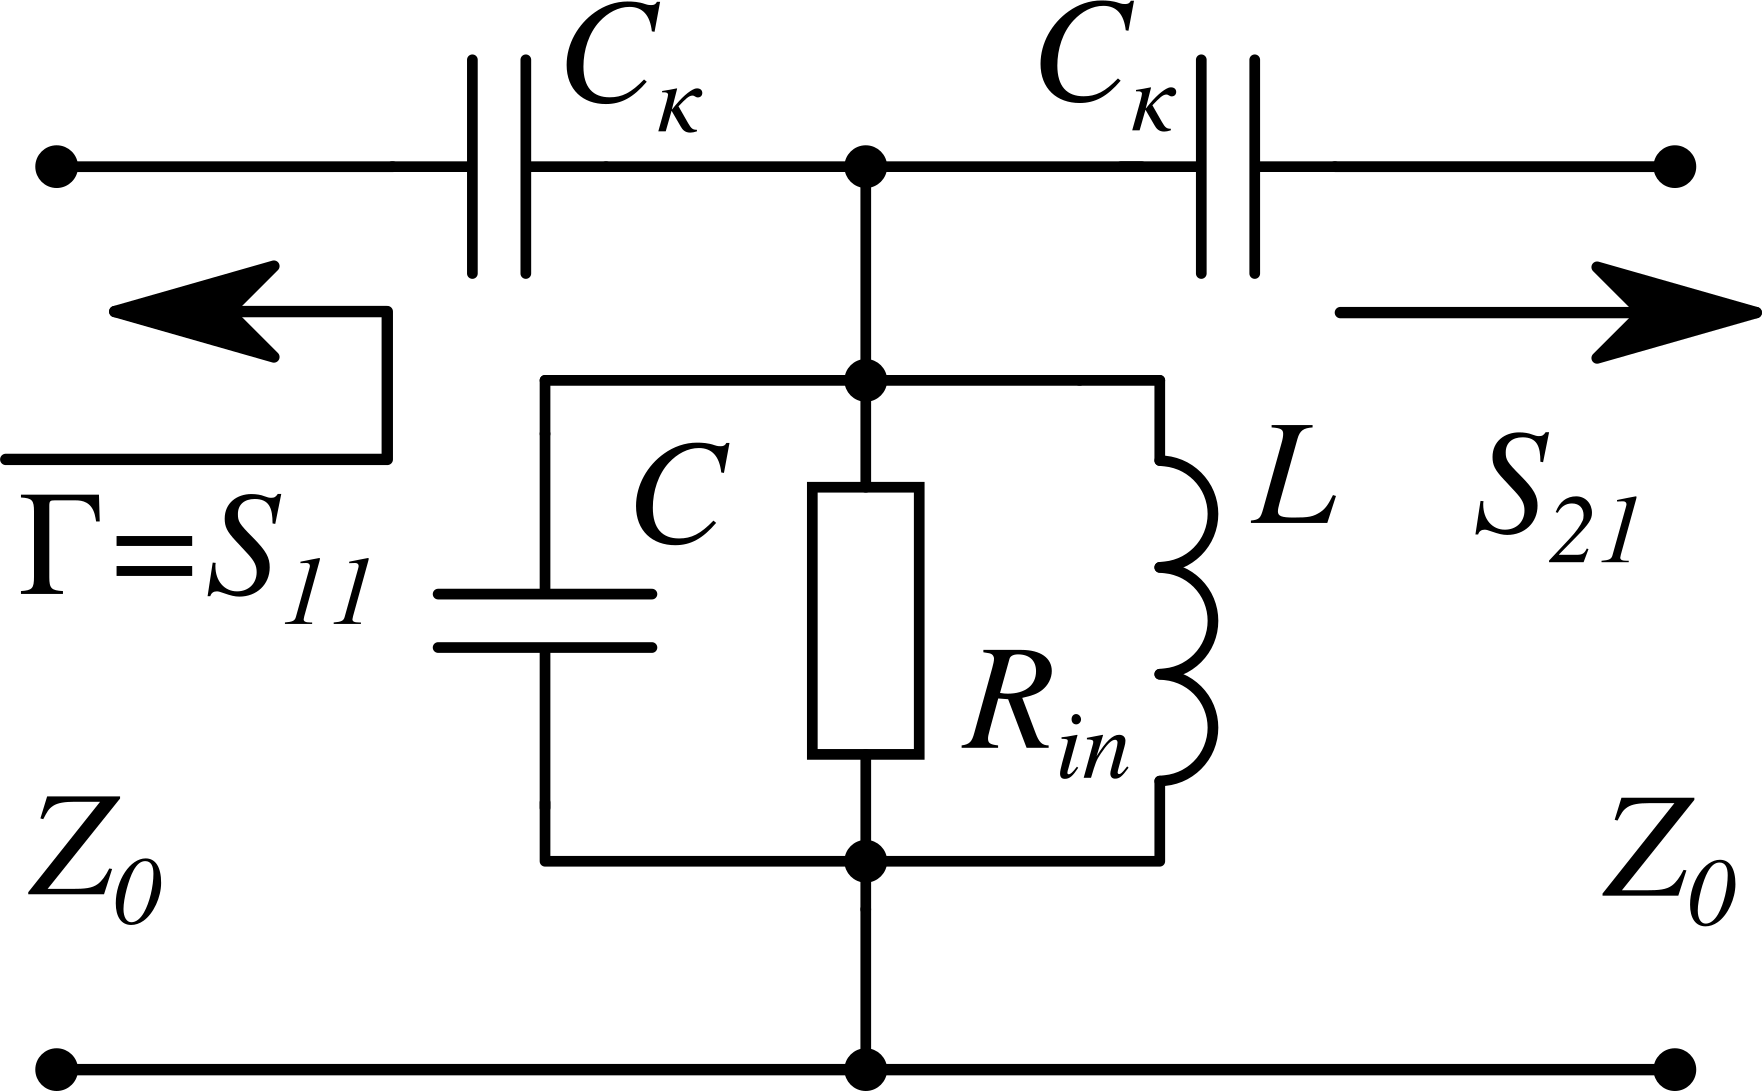
\includegraphics[width=0.5\textwidth]{tl_scheme_series}
\caption{The equivalent circuit for the embedded resonator.}
\label{fseries_tl}
\end{figure}
\begin{figure}[h]
\centering
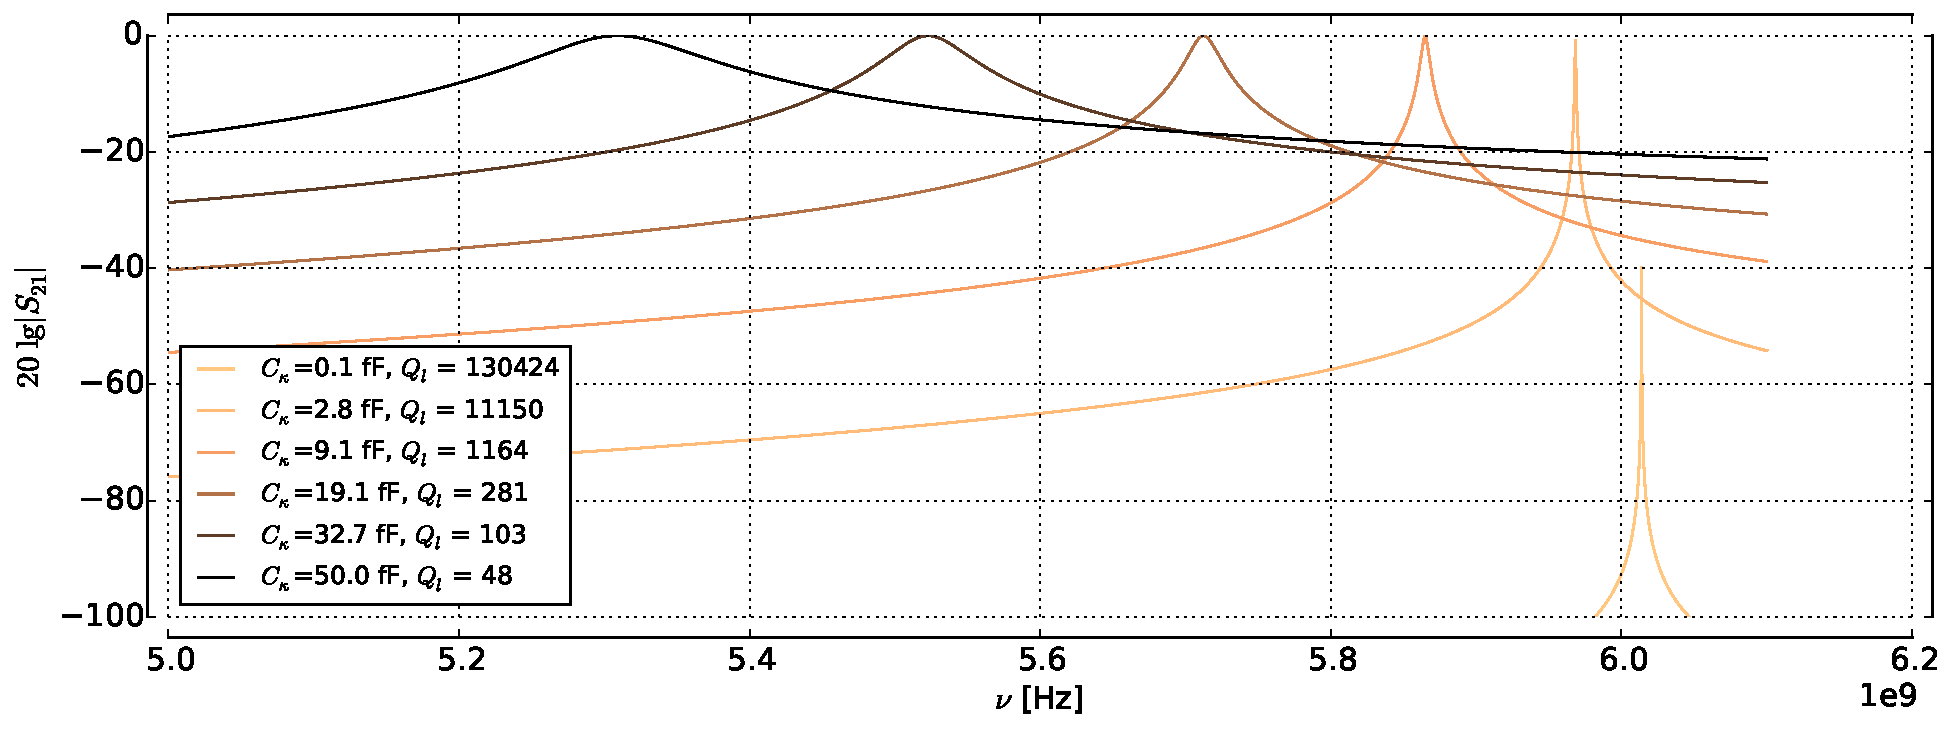
\includegraphics[width=0.9\textwidth]{S21s_series}
\caption{$S_{21}$ for the series configuration. Loaded Q-factors were calculated  via analytic expression similar to \eqref{eq:Q_l}.}
\label{fS21s_series}
\end{figure}

For this kind of connection of the resonator to the transmission line \eqref{eT} is now not valid (however, \eqref{eGamma} still holds true). To calculate transmission in this case one can find the transmission matrix and then convert it to the S-matrix. For studied case one can get the following $ABCD$-matrix\cite{pozar2012}
\begin{equation}
\hat T = \rbrkt{\begin{matrix}
A & B \\
C & D
\end{matrix}} = \rbrkt{\begin{matrix}
1 + \frac{1/i\omega C_\kappa}{Z_{res}} & 2/i\omega C_\kappa - \frac{\omega^2 C_\kappa^2}{Z_{res}} \\
1/Z_{res} &  1 + \frac{1/i\omega C_\kappa}{Z_{res}} 
\end{matrix}},
\end{equation}
where $Z_{res} = R_{in}||i\omega L || 1/i\omega C$. The corresponding $S_{21}$ is  plotted in \autoref{fS21s_series} and can be calculated as\cite{pozar2012} 
\begin{equation}
S_{21} = \frac{2}{A+B/Z_0 +CZ_0 + D}
\end{equation}

\appendix

\chapter{Dephasing or Does the density matrix really exist?}

There are two ways of describing dephasing. One is developed from the system-bath approach (Lindbladian master equation) and the other comes from the stochastic Schrödinger equation. However the results of the latter deviate from the results of the latter for the experiment of spin-echo for single qubit. Here this problem will be described in detail.

\section{Quantum derivation of dephasing}

For the derivation of the phase-destroying process in a quantum way the system-bath interaction Hamiltonian part is chosen as
\[
\mathcal{\hat H}_{sb} = \hat \sigma_z \otimes \hat O_b, 
\]
where $\hat O_b$ is an arbitrary bath operator. From this interaction a master equation it then developed:
\[
\partial_t \hat \rho_s = \frac{i}{\hbar}[\hat \rho_s, \mathcal{\hat H}_s] + \gamma_\phi (\hat \sigma_z \hat \rho_s \hat \sigma_z - \hat \rho_s)
\]

The dynamics of this equation can be seen on



\bibliographystyle{ugost2008}
\bibliography{report.bib}
\end{document}